\documentclass[14pt]{extbook}
\usepackage{multicol, enumerate, enumitem, hyperref, color, soul, setspace, parskip, fancyhdr} %General Packages
\usepackage{amssymb, amsthm, amsmath, bbm, latexsym, units, mathtools} %Math Packages
\everymath{\displaystyle} %All math in Display Style
% Packages with additional options
\usepackage[headsep=0.5cm,headheight=12pt, left=1 in,right= 1 in,top= 1 in,bottom= 1 in]{geometry}
\usepackage[usenames,dvipsnames]{xcolor}
\usepackage{dashrule}  % Package to use the command below to create lines between items
\newcommand{\litem}[1]{\item#1\hspace*{-1cm}\rule{\textwidth}{0.4pt}}
\pagestyle{fancy}
\lhead{Makeup Progress Quiz -1}
\chead{}
\rhead{Version A}
\lfoot{7547-2949}
\cfoot{}
\rfoot{Fall 2020}
\begin{document}

\begin{enumerate}
\litem{
Solve the rational equation below. Then, choose the interval(s) that the solution(s) belongs to.\[ \frac{-6}{7x -3} + -4 = \frac{2}{-42x + 18} \]\begin{enumerate}[label=\Alph*.]
\item \( x \in [-0.67,-0.6] \)
\item \( x_1 \in [0.08, 0.22] \text{ and } x_2 \in [-0.77,1.23] \)
\item \( x \in [0.23,1.23] \)
\item \( \text{All solutions lead to invalid or complex values in the equation.} \)
\item \( x_1 \in [-0.67, -0.6] \text{ and } x_2 \in [-0.77,1.23] \)

\end{enumerate} }
\litem{
Choose the graph of the equation below.\[ f(x) = \frac{-1}{(x - 2)^2} - 2 \]\begin{enumerate}[label=\Alph*.]
\begin{multicols}{2}\item 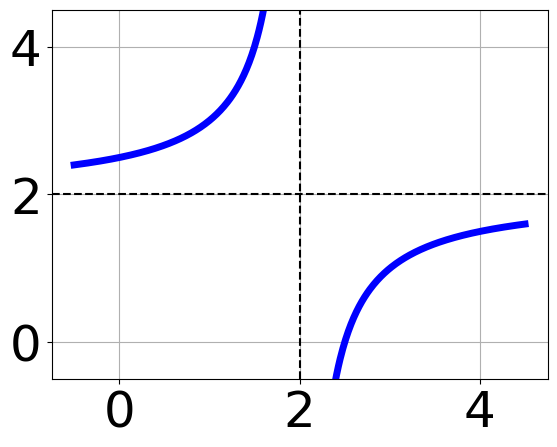
\includegraphics[width = 0.3\textwidth]{../Figures/rationalEquationToGraphCopyAA.png}\item 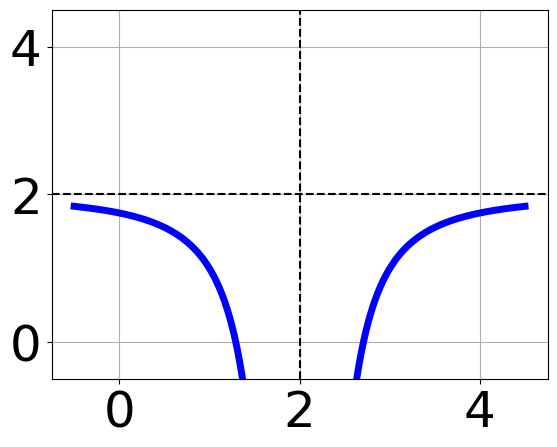
\includegraphics[width = 0.3\textwidth]{../Figures/rationalEquationToGraphCopyBA.png}\item 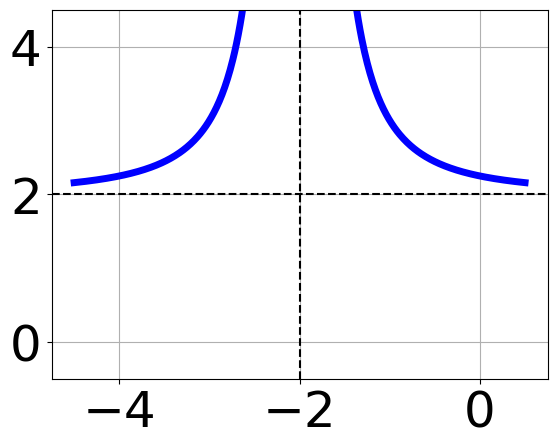
\includegraphics[width = 0.3\textwidth]{../Figures/rationalEquationToGraphCopyCA.png}\item 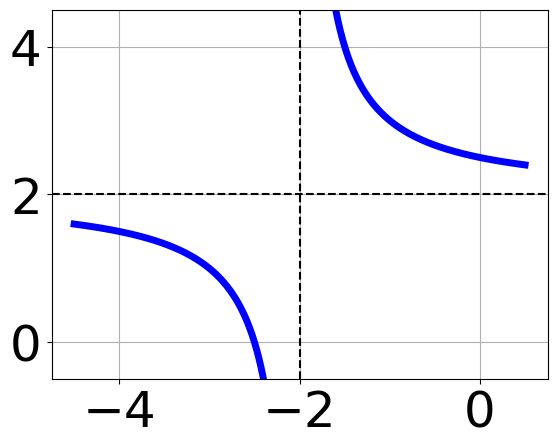
\includegraphics[width = 0.3\textwidth]{../Figures/rationalEquationToGraphCopyDA.png}\end{multicols}\item None of the above.
\end{enumerate} }
\litem{
Solve the rational equation below. Then, choose the interval(s) that the solution(s) belongs to.\[ \frac{98}{-112x + 112} + 1 = \frac{98}{-112x + 112} \]\begin{enumerate}[label=\Alph*.]
\item \( x_1 \in [-4, 0] \text{ and } x_2 \in [1,2] \)
\item \( x \in [-4,0] \)
\item \( x_1 \in [0, 4] \text{ and } x_2 \in [1,2] \)
\item \( \text{All solutions lead to invalid or complex values in the equation.} \)
\item \( x \in [1.0,2.0] \)

\end{enumerate} }
\litem{
Determine the domain of the function below.\[ f(x) = \frac{3}{15x^{2} -24 x + 9} \]\begin{enumerate}[label=\Alph*.]
\item \( \text{All Real numbers except } x = a, \text{ where } a \in [0.44, 0.71] \)
\item \( \text{All Real numbers.} \)
\item \( \text{All Real numbers except } x = a \text{ and } x = b, \text{ where } a \in [8.87, 9.33] \text{ and } b \in [14.87, 15.1] \)
\item \( \text{All Real numbers except } x = a \text{ and } x = b, \text{ where } a \in [0.44, 0.71] \text{ and } b \in [0.8, 1.45] \)
\item \( \text{All Real numbers except } x = a, \text{ where } a \in [8.87, 9.33] \)

\end{enumerate} }
\litem{
Choose the equation of the function graphed below.
\begin{center}
    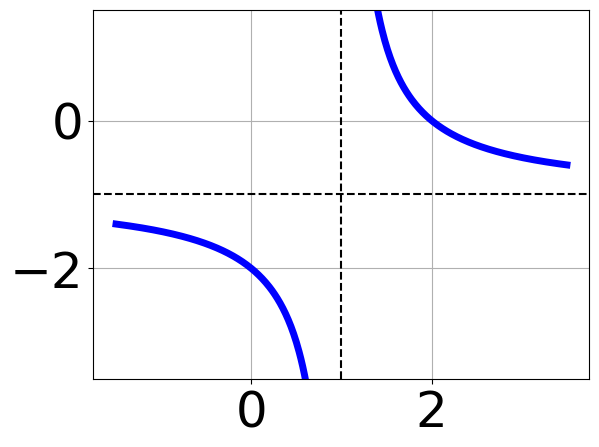
\includegraphics[width=0.5\textwidth]{../Figures/rationalGraphToEquationCopyA.png}
\end{center}
\begin{enumerate}[label=\Alph*.]
\item \( f(x) = \frac{-1}{x - 1} + 3 \)
\item \( f(x) = \frac{1}{(x + 1)^2} + 3 \)
\item \( f(x) = \frac{-1}{(x - 1)^2} + 3 \)
\item \( f(x) = \frac{1}{x + 1} + 3 \)
\item \( \text{None of the above} \)

\end{enumerate} }
\litem{
Determine the domain of the function below.\[ f(x) = \frac{3}{30x^{2} -6 x -36} \]\begin{enumerate}[label=\Alph*.]
\item \( \text{All Real numbers.} \)
\item \( \text{All Real numbers except } x = a, \text{ where } a \in [-37, -29] \)
\item \( \text{All Real numbers except } x = a, \text{ where } a \in [-2, 0] \)
\item \( \text{All Real numbers except } x = a \text{ and } x = b, \text{ where } a \in [-37, -29] \text{ and } b \in [29, 31] \)
\item \( \text{All Real numbers except } x = a \text{ and } x = b, \text{ where } a \in [-2, 0] \text{ and } b \in [-0.8, 5.2] \)

\end{enumerate} }
\litem{
Choose the equation of the function graphed below.
\begin{center}
    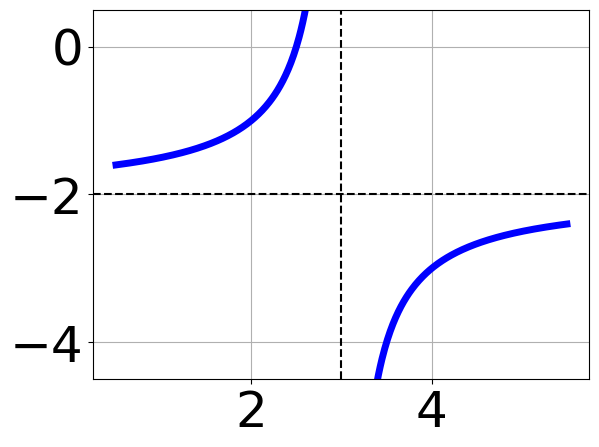
\includegraphics[width=0.5\textwidth]{../Figures/rationalGraphToEquationA.png}
\end{center}
\begin{enumerate}[label=\Alph*.]
\item \( f(x) = \frac{1}{x - 3} - 4 \)
\item \( f(x) = \frac{1}{(x - 3)^2} - 4 \)
\item \( f(x) = \frac{-1}{(x + 3)^2} - 4 \)
\item \( f(x) = \frac{-1}{x + 3} - 4 \)
\item \( \text{None of the above} \)

\end{enumerate} }
\litem{
Solve the rational equation below. Then, choose the interval(s) that the solution(s) belongs to.\[ \frac{-7x}{-7x + 2} + \frac{-6x^{2}}{28x^{2} -43 x + 10} = \frac{3}{-4x + 5} \]\begin{enumerate}[label=\Alph*.]
\item \( x \in [1.03,2.15] \)
\item \( \text{All solutions lead to invalid or complex values in the equation.} \)
\item \( x_1 \in [-1.12, 0.7] \text{ and } x_2 \in [-0.32,0.42] \)
\item \( x_1 \in [-1.12, 0.7] \text{ and } x_2 \in [0.87,1.03] \)
\item \( x \in [-0.17,1.08] \)

\end{enumerate} }
\litem{
Choose the graph of the equation below.\[ f(x) = \frac{1}{x + 1} + 3 \]\begin{enumerate}[label=\Alph*.]
\begin{multicols}{2}\item 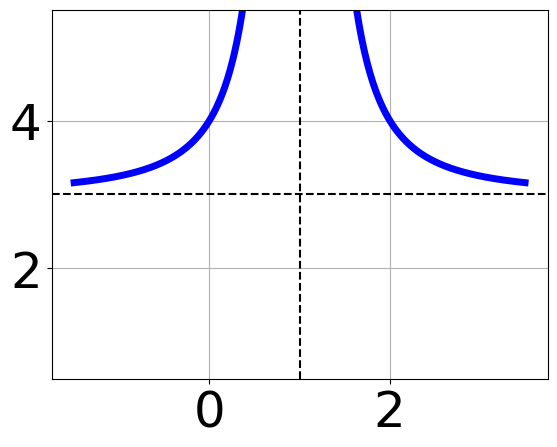
\includegraphics[width = 0.3\textwidth]{../Figures/rationalEquationToGraphAA.png}\item 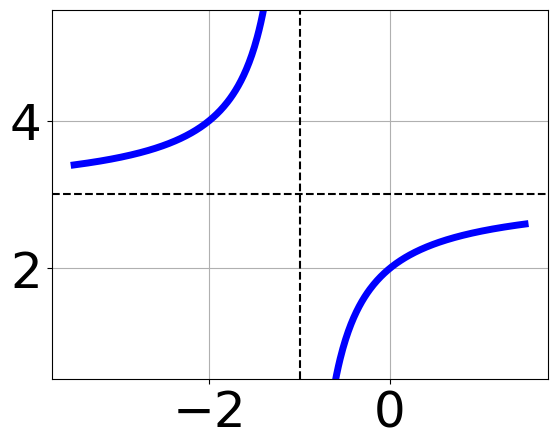
\includegraphics[width = 0.3\textwidth]{../Figures/rationalEquationToGraphBA.png}\item 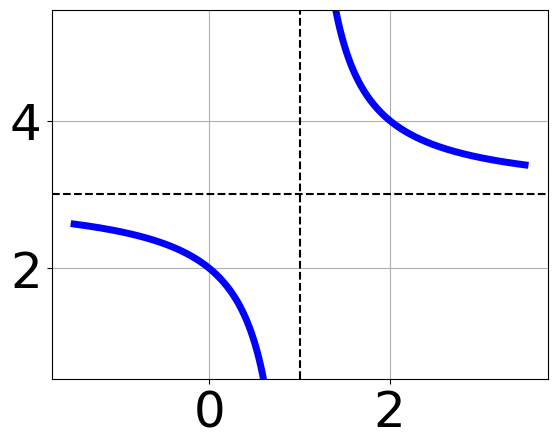
\includegraphics[width = 0.3\textwidth]{../Figures/rationalEquationToGraphCA.png}\item 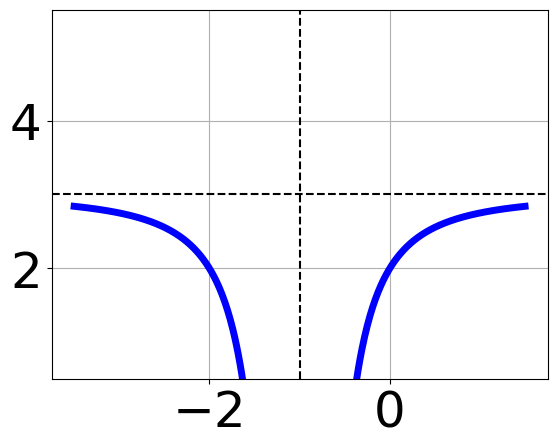
\includegraphics[width = 0.3\textwidth]{../Figures/rationalEquationToGraphDA.png}\end{multicols}\item None of the above.
\end{enumerate} }
\litem{
Solve the rational equation below. Then, choose the interval(s) that the solution(s) belongs to.\[ \frac{6x}{7x + 2} + \frac{-7x^{2}}{-42x^{2} +2 x + 4} = \frac{-3}{-6x + 2} \]\begin{enumerate}[label=\Alph*.]
\item \( \text{All solutions lead to invalid or complex values in the equation.} \)
\item \( x_1 \in [-0.76, 0.14] \text{ and } x_2 \in [-1.12,0.47] \)
\item \( x \in [0.53,1.03] \)
\item \( x \in [0.3,0.48] \)
\item \( x_1 \in [-0.76, 0.14] \text{ and } x_2 \in [0.74,3.18] \)

\end{enumerate} }
\end{enumerate}

\end{document}